\documentclass{article}
\usepackage[margin=1in]{geometry}
\usepackage{xspace} % use \xspace if you have spacing issues in your macros
\usepackage{fancyvrb} % Allows us to use Fancy Verbatim environments
\usepackage{hyperref}
\usepackage{listings}
\usepackage{graphicx}
\usepackage{enumitem}
\usepackage[toc,page]{appendix}
\usepackage{amsfonts}
\usepackage{amsmath}
\usepackage{amsthm}
\usepackage{commath}
\usepackage{color}
\usepackage[svgnames]{xcolor}
\usepackage{tikz}

\newcommand{\AsAnAside}{\footnotesize}
\newcommand{\code}[1]{{\tt#1}}

\newcommand{\FlashOfTheFuture}{ExaFLASH\xspace}

\newcommand{\ie}{\textit{i.e.}}   % use always with comma following: \ie,
\newcommand{\etc}{etc.\xspace}  % or: {\emph{etc.}\xspace}
\newcommand{\eg}{\textit{e.g.}}   % use always with comma following: \eg,
\newcommand{\N}                 {{\mathbb N}}
\newcommand{\Z}                 {{\mathbb Z}}
\newcommand{\Q}                 {{\mathbb Q}}
\newcommand{\R}                 {{\mathbb R}}
\newcommand{\C}                 {{\mathbb C}}
\newcommand{\F}                 {{\mathbb F}}

\newcommand{\TeamStarting}      {\textsc{TeamStarting}}
\newcommand{\TeamIdle}          {\textsc{TeamIdle}}
\newcommand{\TeamRunningOpen}   {\textsc{TeamRunningOpen}}
\newcommand{\TeamRunningClosed} {\textsc{TeamRunningClosed}}
\newcommand{\TeamRunningNoMoreWork} {\textsc{TeamRunningNoMoreWork}}
\newcommand{\TeamTerminating}   {\textsc{TeamTerminating}}

\newcommand{\ThreadStarting}    {\textsc{ThreadStarting}}
\newcommand{\ThreadIdle}        {\textsc{ThreadIdle}}
\newcommand{\ThreadComputing}   {\textsc{ThreadComputing}}
\newcommand{\ThreadWaiting}     {\textsc{ThreadWaiting}}
\newcommand{\ThreadTerminating} {\textsc{ThreadTerminating}}

\newcommand{\spelledoutOR}   {orchestration runtime\xspace}
\newcommand{\spelledoutOS}   {orchestration system\xspace}

\newcommand{\shortOR}   {OR\xspace}
\newcommand{\shortOS}   {OS\xspace}

\newcommand{\OR}        {\shortOR}
\newcommand{\OS}        {\shortOS}

\newcommand{\taskroutine}        {task routine\xspace}
\newcommand{\taskroutines}       {task routines\xspace}
\newcommand{\Taskroutines}       {Task routines\xspace}
\newcommand{\actionroutine}        {action routine\xspace}       %fka task routine
\newcommand{\actionroutines}       {action routines\xspace}
\newcommand{\job}                {\textbf{job}\xspace}  % == \taskroutine execution ?
\newcommand{\jobs}               {\textbf{jobs}\xspace}  % == \taskroutine executions ?



% No automatic indenting
\setlength\parindent{0pt}

% Set spacing between items in itemize/enumerate
\setlist{itemsep=1pt}

\newenvironment{shrink}{%
\begin{center}
\begin{minipage}{0.8\textwidth}}
{\end{minipage}\end{center}}


\title{Orchestration Runtime Thread Team Design}

\begin{document}

% Setup numbered/referentiable environment for requirements
\theoremstyle{definition} % No italics or spaces
\newtheorem{req}{Req}[section]
\newtheorem{spec}{Spec}[section]

\maketitle

%%%%%----- TECHNICAL SPECIFICATIONS & DESIGN SUBSECTION
\section{Technical Specifications \& Design}
We refer to the statements that appear in this section as technical
specifications, rather than requirements, because these statements are low-level,
directly informed by the design, and how we plan to implement the design.
It is expected that a change in the design, that does not violate the
above requirements, could still require significant changes to the technical
specifications in this section.\\

One main intent of the technical specifications is to highlight \textit{some} of
the key ideas, difficulties, complexities, and subtleties that should be kept in
mind when studying and maintaining the code.  Use, corner, and edge cases
that have been identified are presented as motivation for technical
specifications.  Some statements are made because the correctness of
the design and implementation require that they be satisfied.  For such
requirment statements, proofs are given to explain how we know that the
specification is satisfied by the design and actual implemetation.\\

A thread team is fundamentally event-driven software, and thus its design has
been specified as a finite state machine (FSM).  However, the behavior in a
given state cannot be specified solely by a single qualitative state variable.
Rather, the behavior will depend on a qualitative state variable, which is
called the mode, as well as the quantitative internal state variables $N_i, N_w,
N_c, N_Q$ that respectively keep track of
\begin{itemize}
\item{the number of Idle threads in the team,}
\item{the number of threads that are Waiting for work to be added,}
\item{the number of threads applying a \taskroutine on a unit of work(Computing), and}
\item{the number of units of work in the team's pending work Queue.}
\end{itemize}
Note that the definitions of $N_i, N_w, N_c$ imply that each thread is
always in one and only one of the Idle, Waiting, and Computing states, but that
this EFSM need not track the actual state of each thread --- it is only the
aggregated thread state information that is important.  Therefore, the runtime
is an extended finite state machine (EFSM)
\[
M = (Q, X, I, O, s_0, T)
\]
where
\begin{itemize}
\item{$Q$ is the finite set of qualitative modes,}
\item{$X = \set{(N_i, N_w, N_c, N_Q) \in \Z[0,N_{max}]^3\times\Z_{\ge 0}\,|\,N_i + N_w + N_c =
N_{max}}$ is the set of internal state variables where $N_{max}$ is the
number of threads in the team,}
\item{$I$ is the set of internal and external events,}
\item{$O$ is the set of outputs,}
\item{$s_0 = (q_0, x_0) \in Q \times X$ is the initial state, and}
\item{$T : Q \times X \times I \to Q \times X \times O$ is the Transition
function that is evaluated by the EFSM at each occurrence of an event to
identify the output to be performed as well as the state to which the EFSM must
be transitioned.}
\end{itemize}

Note that the set of all possible states is not $Q \times X$.  There are
elements in that set that the EFSM must not occupy.  See
Specs~\ref{spec:Closed_NoWork} and~\ref{spec:NoMoreWork_NeedThread} for examples
of such prohibited states.  Therefore, the above specification of $T$ is only
correct if we assume that the output associated with such prohibited states is
to inform client code of an error so that the EFSM can be terminated.\\

The set $Q$ contains the modes
\begin{itemize}
\item{\TeamIdle --- all threads Idle and no work in the queue}
\item{\TeamRunningOpen --- a \taskroutine has been given to the team. Units of work
on which to apply the \taskroutine can still be given to the team (\textit{i.e.} an
execution cycle has been started)}
\item{\TeamRunningClosed --- a \taskroutine is being applied, but no more units
of work can be given to the team in the current execution cycle}
\item{\TeamRunningNoMoreWork --- a \taskroutine is being applied, no more
units of work can be given, and the team has identified that the \taskroutine has
already been applied to, or is currently being applied to, all units of work given
to the team for the current execution cycle}
%\item{\TeamTerminating --- the client has indicated that it no longer needs the team.}
\end{itemize}

The set $I$ of events is the union of events triggered by clients through the
team's interface
\begin{itemize}
\item{\texttt{startTask} --- give the team a \taskroutine, and activate a given number of the
$N_{max}$ Idle threads in the team to work on it}
\item{\texttt{increaseThreadCount} --- activate a given number of Idle threads in the
team so that they can start working on the \taskroutine as well}
\item{\texttt{enqueue} --- give the team a unit of work on which to apply its
\taskroutine}
\item{\texttt{closeTask} --- indicate (without blocking the caller) to the team
that no more units of work will be given for the current \taskroutine}
%\item{\texttt{$\sim$ThreadTeam} --- thread team no longer needed}
\end{itemize}
with the set of events triggered internally
\begin{itemize}
\item{\texttt{activateThread} --- wake an Idle thread to participate
in applying a \taskroutine to given units of work, look for pending work, and update its
state accordingly}
\item{\texttt{transitionThread} --- wake a thread that is Waiting for work so
that it can evaluate if there is pending work, and update its state accordingly}
\item{\texttt{computationFinished} --- a Computing thread finished applying the team's
\taskroutine to a unit of work and shall evaluate if there is pending work and update
its state accordingly}
%\item{\texttt{threadTerminated} --- emitted by a thread to indicate that it has
%terminated}
\end{itemize}

Note that \texttt{computationFinished} is different from the other events, and it
is important to understand how it is different, as well as how we define it to
make certain that this event does not break the rules of a FSM.  Specifically,
when a thread transitions to Computing it does not sleep or wait on another
event as is the case for Waiting or Idle threads.  Rather, it does work.  Seen
in this light, a state transition in the EFSM that results in a thread becoming
a Computing thread does not terminate until the Computing thread finishes
applying the team's \taskroutine to its current unit of work.  Therefore, we should not
allow any other thread to alter the state of the EFSM until the work is
finished.\\

Therefore, we emphasize that in our design the Computing thread is
\textit{effectively} sleeping while it is applying the team's \taskroutine to a unit of
work and a EFSM state transition can finish when such a thread ``goes to
sleep.''  It is sleeping, not in the sense of no resource usage, but rather from
the perspective of not being an active member of the runtime infrastructure,
while it is computing.  As with Waiting and Idle threads, the Computing threads
need to be awakened by a dedicated event, which is the
\texttt{computationFinished} event.  This event is ``emitted'' by a Computing
thread when it finishes applying a \taskroutine to its current unit of work and can only
be received by the thread itself.\\

The initial state is defined to be
\[
s_0 = \left(q_0, (N_i, N_w, N_c, N_Q)_0\right) = \left(\TeamIdle, (0, 0, 0, 0)\right).
\]

The set $O$ and the transition function $T$ encapsulate the complexity of the
runtime.  A state diagram for the team
that indicates only states and transitions is shown in
Figure~\ref{fig:TeamStateDiagram}.  A similar state diagram for threads in the
team is shown in Figure~\ref{fig:ThreadStateDiagram}.  These figures are
intended only to aid in understanding the design of the runtime. \\

The design and implementation philosophy of the EFSM was to emphasize
correctness and maintainability.  One important consequence was to create a
design that accounts for almost all\footnote{There are a few states,
transitions, and events that the EFSM \textit{must} avoid so that the EFSM
functions properly.  For such cases, proofs have been given to show correctness
of the design.  A few examples of some prohibited states are given in
Specs~\ref{spec:Closed_NoWork} and~\ref{spec:NoMoreWork_NeedThread}} possible
states, transitions, and events; even though it could be proven that some
states/transitions/events are precluded from happening by the design itself.
Our design/implementation is hopefully robust and not sensitive to
small design changes.  Also, the mental load associated with working with the
design is lower since we decrease the burden of proving and maintaining
proofs of impossible states/transitions/events.  This is especially important as
the implementation of the thread team cannot make strong assumptions about the
predictability of the order of execution of code and events, which increases the
complexity of such proofs.  This philosophy is ugly in that the code might,
without the developers' knowledge, carry out actions that it shouldn't.  It also
means that we have not completely understood the full behavior of the EFSM.\\

It is important to have in mind some examples of out-of-order execution of the
EFSM.  This list is meant only to clarify what is meant by out-of-order, and to
spur on the identification of other such interesting cases.  This list is
not exhaustive.
\begin{enumerate}
\item{Work could be given to the team, and as a result, the
\texttt{transitionThread} signal emitted.  However, a Computing thread could
finish its computation and dequeue this unit of work before a Waiting thread
receives the emitted signal.  Waiting threads are programmed so that
they transition back to Waiting, if they find that the queue is empty (See
Figure~\ref{fig:ThreadStateDiagram}).}
\item{When \texttt{startTask} is called with $N$ threads to be activated, $N$
\texttt{activateThread} signals are emitted.  However, if the \job execution is
quick, it is possible that the team's mode could transition all the way back to
Idle, before all of these signals are received.  Therefore, Idle threads are
programmed to determine if a transition out of Idle is in accord with the
present state of the EFSM.}
\end{enumerate}

\begin{figure}[!ht]
\begin{center}
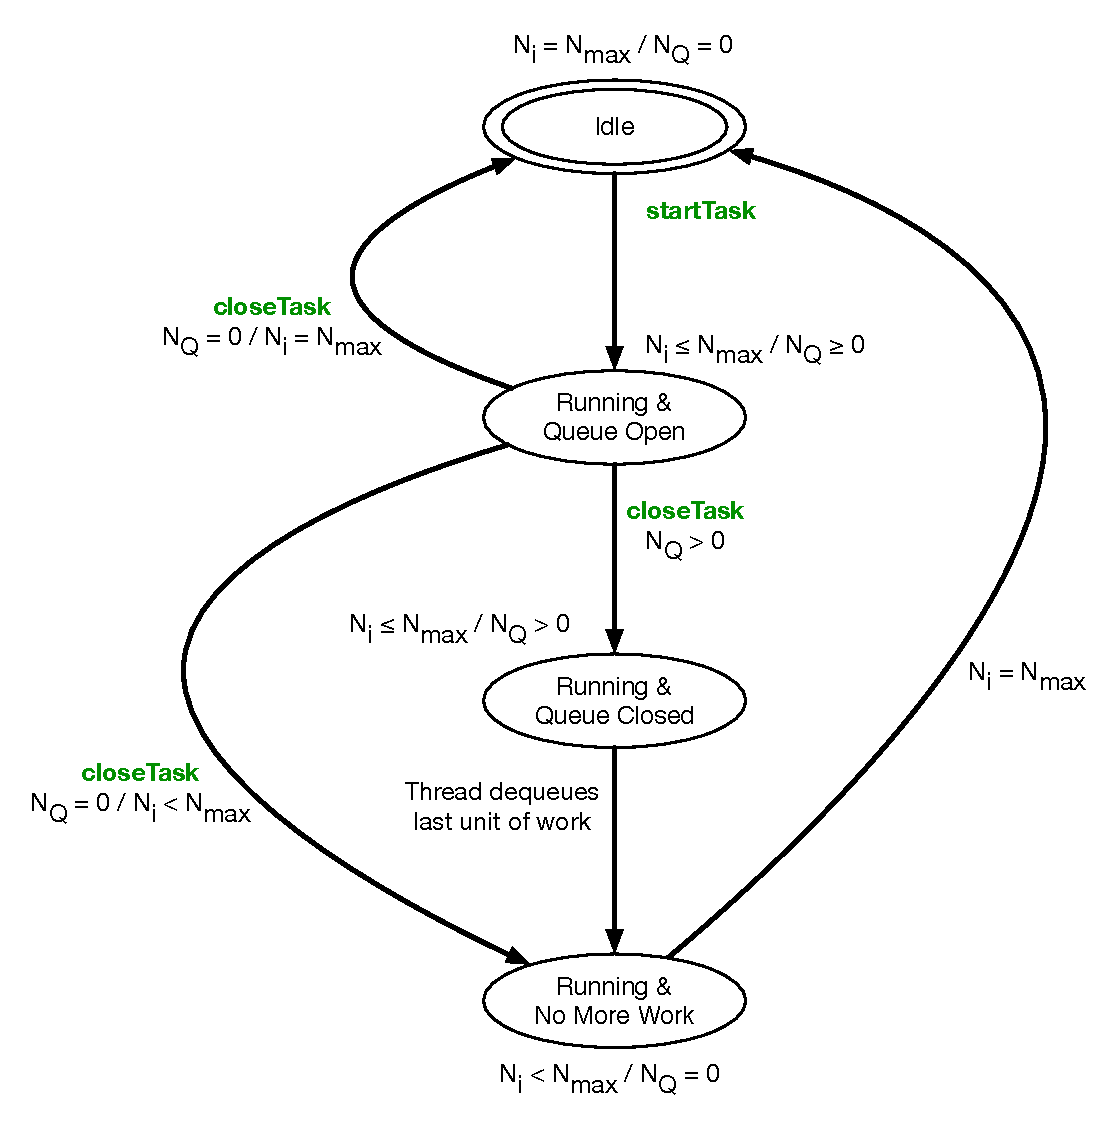
\includegraphics[width=5.0in]{TeamStates.pdf}
\caption[]{}
\label{fig:TeamStateDiagram}
\end{center}
\end{figure}

\begin{figure}[!hp]
\begin{center}
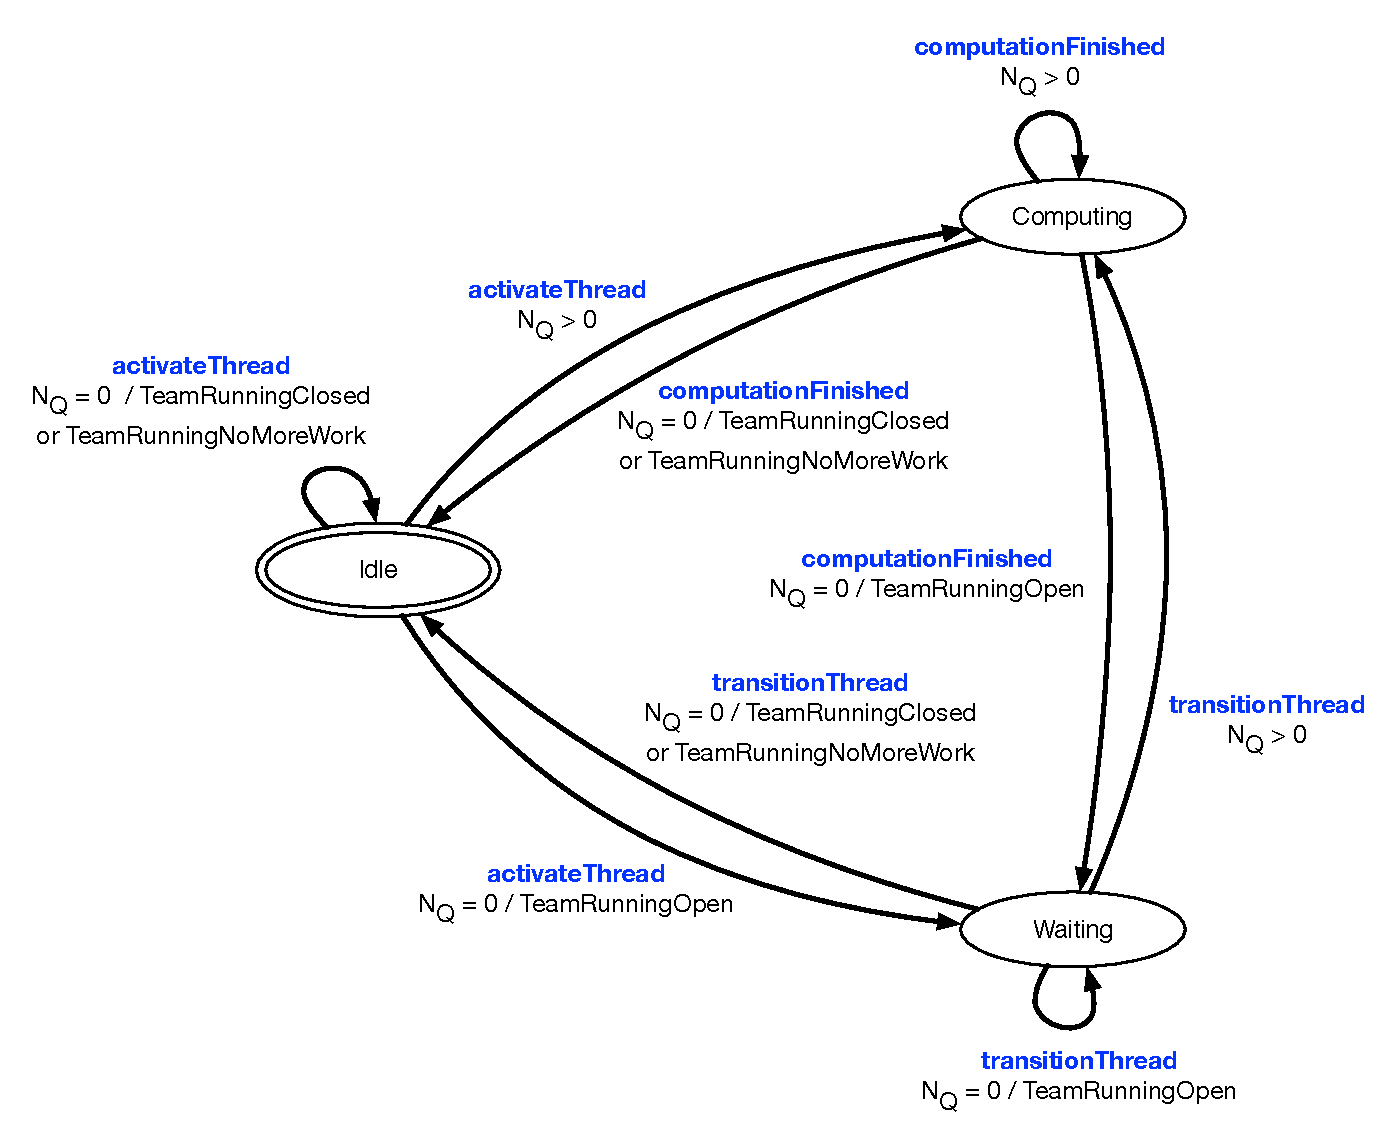
\includegraphics[width=6.5in]{ThreadStatesPersistent.pdf}
\caption[]{}
\label{fig:ThreadStateDiagram}
\end{center}
\end{figure}


\begin{spec}
\label{spec:Runtime_AtomicTransition}
As per the requirements of FSMs, each transition shall be implemented so that
the code executing the transition has sole access to the thread team's state,
during the entirety of the transition.  This implies that no other thread can
alter the state simultaneously, and that transitions are atomic.
\end{spec}
\textbf{Verification:}\hspace{0.125in}  Each thread team has a single,
dedicated mutex that must be acquired to access or alter thread team state
information.  Each transition acquires the mutex either through an explicit
request, or by a thread receiving an event.  The mutex is not released until
the transition is finalized.\\


Given the present implementation, it is important for transitions that
change the mode and emit internal signals, that the code change the mode
\textbf{first}, and then emit the signals.  This prevents the possible
(\textbf{TBC} for pthreads?) case that the signal is emitted and received before
the mode is correctly transitioned, which would violate
Spec~\ref{spec:Runtime_AtomicTransition}, and cause the responding thread
to react to the signal is a way that is potentially not in accord with the true
mode of the EFSM.

\begin{spec}
A thread team shall maintain a set of pending units of work, and all threads in a
thread team shall be able to check the set of pending units of work.  In
addition, each thread in the team shall be able to claim ownership of a single
unit of work by removing it from the set, with the understanding that the thread
itself is responsible for applying the team's \taskroutine to that unit of work.  It
shall be impossible for two threads to simultaneously claim ownership of the
same unit of work.
\end{spec}
\textbf{Verification:}\hspace{0.125in}  Pending work queues implemented as
stated.  As per Spec~\ref{spec:Runtime_AtomicTransition}, dequeueing of units of
work are only done after obtaining the mutex and no handle to dequeued units of
work remain.  Therefore, the only thread that can access a dequeued unit of work
is the thread that dequeued it.
\begin{spec}
All threads that transition to Idle must wait for the \texttt{activateThread}
event.  This includes threads in Idle that receive the \texttt{activateThread}
event but remain in Idle, as well as all threads that are \textit{set} into the
Idle state, when the EFSM is set up in the initial state.
\label{spec:IdleActivateThread}
\end{spec}

\begin{spec}
External code shall only be able to decrease $N_i$ through the
\texttt{startTask} and \texttt{increaseThreadCount} events, and the runtime shall
be implemented such that a request to activate $i$ threads results in an error
if $i$ exceeds the number of Idle threads that are available for activation.
Note that this technical specification is consistent with
Req~\ref{req:ThreadBalance}.
\end{spec}
\textbf{Verification:}\hspace{0.125in}  In the present design, this requirement
is important because the runtime would emit more \texttt{activateThread} signals
than there are threads to receive them.  Because teams allow for thread
publishers/subscribers, undetected signals would amount to a loss of thread
resources at the level of the runtime.  Note that a thread-based implementation
will have a lag between when these events trigger the activation of Idle threads,
and when these threads are actually activated.  The runtime design therefore
tracks the actual number of Idle threads with \texttt{N\_idle\_} = $N_i$, as well
as the number of threads pending activation with \texttt{N\_to\_activate\_}.
When a thread does receive \texttt{activateThread}, it decrements both
\texttt{N\_idle\_} and \texttt{N\_to\_activate\_} by one and increments by one
the internal state variable $N_i, N_w$ or $N_c$ corresponding to the thread's
next state.  To satisfy the requirement, both events throw an error if $i > $
\texttt{N\_idle\_} - \texttt{N\_to\_activate\_}.  No other public thread team
methods can emit \texttt{activateThread}.

\begin{spec}
\label{spec:Runtime_OneWait}
The interface of the thread team shall contain a \texttt{wait} method, so that
for each \taskroutine execution, the execution of an external thread that calls
\texttt{wait} is blocked until the termination of the \taskroutine.  This interface
shall allow for at most one such thread to block its execution with this method
during each \taskroutine execution.
\end{spec}
\textbf{Verification:}\hspace{0.125in}  Implemented a flag
\texttt{isWaitBlocking\_} to track if a thread has already called \texttt{wait}.

\begin{spec}
To maintain a simple design, client code shall only be allowed to attach and
detach thread subscribers when the team is in the {\TeamIdle} mode.  The same
requirement applies for work subscribers.
\end{spec}
\textbf{Verification:}\hspace{0.125in} Implemented directly as stated.

\begin{spec}
In the original designs, the Team state machine also contained a
{\TeamTerminating} mode.  The transition to this mode was allowed only from
{\TeamIdle}, and was triggered by initiating the destruction of the team.  While
sensible, this design was flawed since a runtime error that occurs with the team
in any state could trigger the destruction of the team.  Therefore, the
termination of the EFSM and the clean-up of its resources shall be possible from
any state.
\end{spec}
\textbf{Verification:}\hspace{0.125in}  The destructor does not do any error
checking to confirm that destruction was called with the EFSM in any particular
state.  Also, the destructor assumes that there are Idle, Waiting, and Computing
threads at the time of calling.  For the Idle and Waiting threads, it signals
them to terminate; Computing threads, it waits for them to finish their work and
discover that they should terminate.

\begin{spec}
\label{spec:Runtime_AwakenOnNoMoreWork}
All transitions to {\TeamRunningNoMoreWork} from a different mode shall awaken
all Waiting threads so that they can transition to Idle.
\end{spec}
\textbf{Verification:}\hspace{0.125in}  Implemented directly as stated.

\begin{spec}
\label{spec:Runtime_CompMustEnqueue}
Upon emitting/receiving the \texttt{computationFinished} signal, a Computing
thread shall enqueue the unit of work that it just finished applying the team's
\taskroutine to, with the team's work subscriber, if the team has a work subscriber.
\end{spec}
\textbf{Verification:}\hspace{0.125in}  Implemented directly as stated.

\begin{spec}
\label{spec:Runtime_IdleOutput}
All transitions to {\TeamIdle} from a different mode shall
\begin{itemize}
\item{call the \texttt{closeTask} method of the team's work subscriber (if it
has a work subscriber) and }
\item{unblock the external thread that called \texttt{wait}, if such a thread
exists.}
\end{itemize}
If the transition to {\TeamIdle} is handled by a Computing thread, then the
Computing thread shall enqueue its unit of work
(Spec~\ref{spec:Runtime_CompMustEnqueue}) prior to calling \texttt{closeTask}.
Note that this specification is not applicable to the case of \textit{setting}
the EFSM into its initial state.
\end{spec}
\textbf{Verification:}\hspace{0.125in}  Implemented directly as stated.

\begin{spec}
\label{spec:Runtime_IdleToIdle}
It is possible for an Idle thread to receive the \texttt{activateThread} event
when the team does not need threads to be activated (\textit{i.e.} the mode is
\TeamIdle \footnote{Consider a team that is both a thread publisher and
subscriber.  It is possible for the team to finish its work and transition to
{\TeamIdle} before its publisher and subscriber finish their work.} or
\TeamRunningNoMoreWork).  To avoid thread resource loss and to promote efficient
execution of the execution cycle's \taskroutines, in this scenario the threads that
receive the unnecessary event shall remain in Idle and call
\texttt{increaseThreadCount(1)} for its thread subscriber if it exists.
\end{spec}
\textbf{Verification:}\hspace{0.125in} Implemented directly as stated.

\begin{spec}
\label{spec:Runtime_ForwardThreads}
To prevent thread resource loss at the level of the runtime, all threads that
transition to Idle shall call \texttt{increaseThreadCount(1)} of its thread
subscriber, should it exist.  This specification is consistent with
Spec~\ref{spec:Runtime_IdleToIdle}, which could be understood to handle the
special case that an Idle thread transitions to Idle.  Note that this
specification is not applicable to the case of \textit{setting} the EFSM into
its initial state. This technical specification is consistent with
Req~\ref{req:ThreadSubPub}.
\end{spec}
\textbf{Verification:}\hspace{0.125in} Implemented directly as stated.

\begin{spec}
\label{spec:Runtime_NoEnqueue}
Client code shall only be allowed to give a team a unit of work if the team is
in the mode {\TeamRunningOpen}.  While the runtime could allow clients to give
units of work to a team that is in {\TeamIdle}, with the understanding that the
work would be for the next \taskroutine to be given to the team, there is no known use
case for which this is necessary.  Thus, this specification is motivated by
the goal of simplifying the design.
\end{spec}
\textbf{Verification:}\hspace{0.125in}  The \texttt{enqueue} method is the only
means for giving a unit of work to a team.  Attempts to use this method when the
team is not in {\TeamRunningOpen} result in error.\\

Based on this specification, client code should call \texttt{startTask} on all
thread teams to be used on a \taskroutine before enqueueing work with any of these.  This
practice will help avoid the case where an active work publisher tries to
enqueue work on a work subscriber that is still in the mode \TeamIdle.\\

As a final note, the design accounts for \texttt{transitionThread} events that
occur when no Waiting threads exist.  For each of these, this occurrence is
acceptable, and no output is generated as part of the transition.  This
transition is included for the sake of completeness and can occur with the
current implementation when certain outputs broadcast \texttt{transitionThread}.
Unlike for \texttt{activateThread}, it is unimportant that there is no thread to
receive the event.  This is due to the fact that this event exists to inform a
Waiting thread to look for work or that it should determine that it should
transition to Idle.  If there are no Waiting threads because all threads are
Idle, then the team must be in \TeamIdle, (in which case we don't need to
activate threads,) or in \TeamRunningOpen.  In \TeamRunningOpen we wait for
threads to be activated or for \texttt{closeTask} to be called to transition
the team to \TeamIdle.  If all threads are Computing, then these will discover
that there is pending work and the team will stay maximally busy.

%%-- TEAM IDLE SUBSECTION
\subsubsection{{\TeamIdle} State}
\begin{spec}
Similar to Spec~\ref{spec:Runtime_ForwardThreads}, if client code calls the
\texttt{increaseThreadCount} method of a thread team in \TeamIdle, the team shall
forward the pushed thread resources immediately on to its thread subscriber if
it exists.
\end{spec}
\textbf{Verification:}\hspace{0.125in}  Implemented directly as stated.

\begin{spec}
In the {\TeamIdle} mode, the queue shall always be empty, with all threads in the
team in the Idle state.  This implies that no thread can be in the Waiting
state, the Computing state, or terminating, and that all threads are
(Spec~\ref{spec:IdleActivateThread}) waiting to receive the
\texttt{activateThread} event.
\end{spec}
\textbf{Verification:}\hspace{0.125in}  The initial state starts in {\TeamIdle},
and specifies that there is no work in the queue.  Also, all transitions to
{\TeamIdle} only happen if the queue is empty.  Therefore, the pending work
queue is always empty upon entry to \TeamIdle.  Finally, no work can be added to
the queue in the {\TeamIdle} state by Spec~\ref{spec:Runtime_NoEnqueue}.\\

The initial state specifies that all threads are Idle, and transitions to
{\TeamIdle} only happen if the same is true.  Therefore, the claim is true upon
entry to {\TeamIdle}, and all threads are waiting for \texttt{activateThread}.
Responses
\footnote{These cases are being considered if one of these
events be emitted when the team in not Idle, but is received after transitioning
to Idle.  With the current implementation, since all threads would be waiting on
\texttt{activateThread}, no threads would be waiting for the latter two events.}
to \texttt{activateThread}, \texttt{transitionThread}, and
\texttt{computationFinishes} do not transition the thread state and have the
responding threads wait for \texttt{activateThread}.  Any attempt to
transition a thread terminates with the thread in Idle.

\begin{spec}
It would seem to be sensible to insist that an external thread cannot call
\texttt{wait} for a team that is in \TeamIdle.  However, it is possible that a
runtime execution cycle could finish and transition a team back to {\TeamIdle},
before an external thread has the chance to call \texttt{wait}.  Therefore, the
\texttt{wait} method shall be enabled in {\TeamIdle} and shall terminate immediately to avoid
unnecessary blocking of the calling thread.  This does allow for
client code to superfluously call \texttt{wait} before the first execution cycle
is run and multiple times between cycles, both of which are logical errors.
\end{spec}
\textbf{Verification:}\hspace{0.125in}  Implemented directly as stated and in
accord with Spec~\ref{spec:Runtime_OneWait}.

%%-- TEAM RUNNING & OPEN SUBSECTION
\subsubsection{\TeamRunningOpen}
\begin{spec}
It would seem sensible to insist that an external thread cannot call
\texttt{wait} during a given execution cycle, unless the \texttt{closeTask} event
has already been issued for the same cycle.  Consider the case of two
team one of which is the work publisher for the other.  As per
Spec~\ref{spec:Runtime_IdleOutput}, when the publisher team transitions to
{\TeamIdle}, it calls the subscriber's \texttt{closeTask} method to inform the
subscriber that it will not be given more work.  This implies that the external
thread that triggers an execution cycle with the runtime does not know when
\texttt{closeTask} is called, and could call \texttt{wait} before this
event occurs.  Hence, a thread team in the state {\TeamRunningOpen} shall allow
for a thread to call \texttt{wait}.
\end{spec}
\textbf{Verification:}\hspace{0.125in}  Implemented directly as stated.

%%-- TEAM RUNNING & CLOSED SUBSECTION
\subsubsection{\TeamRunningClosed}
\begin{spec}
\label{spec:Closed_Transition}
If a team is in mode \TeamRunningClosed, then every thread that transitions to
Computing shall check if $N_Q = 0$ as part of the transition, and after
dequeueing the unit of work on which it will apply its team's \taskroutine.  If $N_Q =
0$, then during the same transition (and therefore before applying the \taskroutine to
the dequeued unit of work) the thread shall change the mode to
\TeamRunningNoMoreWork.
\end{spec}
\textbf{Verification:}\hspace{0.125in}  A thread can be transitioned to
Computing from the Idle, Waiting, and Computing state.  If the mode is
{\TeamRunningClosed}, $N_Q = 1$, and a
thread receives any of the \texttt{activateThread}, \texttt{transitionThread},
or \texttt{computationFinished} events, then the induced transitions always changes
the mode to \TeamRunningNoMoreWork.  No other events result in decreasing $N_Q$
to zero in \TeamRunningClosed.

\begin{spec}
\label{spec:Closed_NoWork}
The transition from {\TeamRunningClosed} to \TeamRunningNoMoreWork (which is the
only transition possible for this mode,) is triggered internally by the active
thread that dequeues the last unit of work (Spec~\ref{spec:Closed_Transition}).
To avoid deadlock, the design of the runtime shall be such that the
EFSM cannot be in mode {\TeamRunningClosed} with $N_Q = 0$.  It is not
necessarily an error if $N_i = N_{max}$ in {\TeamRunningClosed}, as the team
could be a thread subscriber and have a thread activated by its publisher, so
that the team could eventually dequeue elements and determine that there is no
more work.
\end{spec}
\textbf{Verification:}\hspace{0.125in}  The only transition to
{\TeamRunningClosed} is from {\TeamRunningOpen}, which only occurs if $N_Q > 0$.
Hence, the specification is satisfied upon entry into the mode.  The value of
$N_Q$ can decrease in this mode only when a thread transitions to the Computing
state.   By Spec~\ref{spec:Closed_Transition}, the EFSM mode is transitioned to
{\TeamRunningNoMoreWork} as part of every transition that results in $N_Q = 0$.

%%-- TEAM RUNNING & NO MORE WORK SUBSECTION
\subsubsection{\TeamRunningNoMoreWork}
The only transitions into {\TeamRunningNoMoreWork}
are from {\TeamRunningOpen} and \TeamRunningClosed.

\begin{spec}
\label{spec:NoMoreWork_NoWork}
If a team is in \TeamRunningNoMoreWork, then it shall always be true that $N_Q =
0$.
\end{spec}
\textbf{Verification:}\hspace{0.125in}
Since both methods of transition into {\TeamRunningNoMoreWork} only occur if $N_Q = 0$,
the specification is satisfied upon entry to the mode.  The only means to
increase $N_Q$ is by adding work \textit{via} \texttt{enqueue}, which is
prohibited in {\TeamRunningNoMoreWork} by Spec~\ref{spec:Runtime_NoEnqueue}.

\begin{spec}
\label{spec:NoMoreWork_TransitionToIdle}
If a team is in mode \TeamRunningNoMoreWork, then the last thread to transition
to Idle shall change the mode to \TeamIdle.  This transition is valid as $N_i =
N_{max}$ necessarily at the transition and by Spec~\ref{spec:NoMoreWork_NoWork}
it is certain that $N_Q = 0$.
\end{spec}
\textbf{Verification:}\hspace{0.125in}  If the transition to
{\TeamRunningNoMoreWork} is from \TeamRunningOpen, then $N_w > 0$ or $N_c > 0$
(to the contrary, $N_Q = 0$ and $N_i = N_{max}$ so that the transition is to
\TeamIdle).  If the transition is from \TeamRunningClosed, then it follows from
Spec~\ref{spec:Closed_Transition} that $N_c > 0$.  Therefore, upon entry to the
mode, there is at least one thread that could transition to Idle.  Since
satisfaction of Spec~\ref{spec:NoMoreWork_NoWork} implies that $N_Q = 0$, all
Computing threads will determine that there is no more work
upon finishing the application of the team's
\taskroutine to the current unit of work, and threads will
subsequently transition to Idle.  Similarly, satisfaction of
Spec~\ref{spec:Runtime_AwakenOnNoMoreWork} implies that all threads in the Wait
state will be awakened, determine that there is no work, and transition to Idle
as well.  All non-active threads will eventually transition to Idle.
Given this and the fact that the reception of \texttt{activateThread} events are
effectively ignored by Idle threads, we conclude that there will be a last
thread that transitions to Idle.  This thread is programmed to transition the
mode to \TeamIdle.

\begin{spec}
\label{spec:NoMoreWork_NeedThread}
The transition from {\TeamRunningNoMoreWork} to \TeamIdle, which is the only
transition out of this mode, occurs when the last non-Idle thread transitions to
Idle (See Spec~\ref{spec:NoMoreWork_TransitionToIdle}).  Therefore, to avoid
deadlock the design of the runtime shall prohibit the EFSM from being in a state
with {\TeamRunningNoMoreWork} and $N_i = N_{max}$.
\end{spec}
\textbf{Verification:}\hspace{0.125in} As shown in the Verification of
Spec~\ref{spec:NoMoreWork_TransitionToIdle},  $N_i < N_{max}$ upon entry to the
mode. $N_i$ can only decrease by at most one with each thread transition,
which are atomic (Spec~\ref{spec:Runtime_AtomicTransition}). Satisfaction of
Spec~\ref{spec:NoMoreWork_TransitionToIdle} implies that $N_i$ cannot be set to
zero in {\TeamRunningNoMoreWork} without also simultaneously causing the mode to
change to \TeamIdle.  Hence, $N_i < N_{max}$ in {\TeamRunningNoMoreWork} up to
the transition to \TeamIdle.

\end{document}

